\documentclass{article}
\usepackage{blindtext}
\usepackage{fancyhdr}
\usepackage[a4paper, margin=80pt]{geometry}
\usepackage{listings}
\usepackage{graphicx}
\begin{document}
\pagestyle{fancy}
\fancyhead[L]{{\large\bf{0801CS211017}}}
\fancyhead[R]{{\large\bf{Anishiddha Suryawanshi}}}

\begin{center}
{\centering \Large{\textbf{\bf ASSIGNMENT 07\\Mini-Project\\ATM Interface (User side of Banking System)\\}}}\end{center}


\section{Aim}
The Aim of this mini project program is to make interface of User side of the Banking System.
An ATM is a example of User side interface of Banking System.

\section{Working}
There are 2 sides of a Banking System. User side and Bank side. Bank side manages the transaction and keeps the record of user, his login credentials, and their transactions.\\The user side has an Interface from where he can perform actions like checking his Balance, transferring money, withdrawing money, etc while using pin or passwords for safety.

\section{Statistical information :}
Starting date : 14, November, 2022\\
End Date : 20, November, 2022\\
Total Time Taken : 7 days\\
Total Line Of Code (C):  225\\
Number Of Functions (C) : 10\\
Total Line Of Code (Python): 202\\
Number Of Functions (Python) : 10\\

\section{Functions used in this project}
\subsection{mainMenu()}
This function makes a menu appear in front of the user and asks user to select from the provided options.\\Options includes basic user side operations like: Checking balance, Withdraw, Deposit, Change pin, Exit./\subsection{checkBalance()}
This function is called if the user choose to check his balance.This function takes the value of Total Balance as input and prints the total balance.
\subsection{moneyDeposit()}
This function is called if the user choose to Deposit money in his Bank Account.This function takes the value of current Total Balance as input, Adds the Deposit Amount in it, and then prints and  returns the new Total Balance as output.
\subsection{moneyWithdraw()}
This function is called if the user choose to Withdraw money from his Bank Account.This function takes the value of current Total Balance as input,subtracts the withdrawing amount from it, and then prints and  returns the new Total Balance as output.
\subsection{checkPin()}
This function asks the user to enter his pin provided by the Bank at the start and also while performing important tasks like Checking Balance, Withdrawing money, Depositing money, Changing pin etc And checks it with the pin already stored in database (ie,Provided by the bank while opening the bank account for the first time)
\subsection{changePin()}
This function is called when user choose to change his pin. This function takes the value of new pin from the user and updates the value of pin in the database.
\subsection{errorMessage()}
This function is called when the user enters an invalid data. This function provides an Error message "INVALID NUMBER".
\subsection{printReceipt()}
This function is called at the end.This function asks the user if he wants a receipt or not. If yes then it exits the the code while giving the receipt. If no then it exits the code without the receipt.
\subsection{clearScreen()}
 This function itself has a system("cls") function. "cls" means clear screen. This function clears the screen before execution new function providing user with a good interface. 
\subsection{exitMenu()}
This function provides a exiting message at the end.

\section{Code In C language:}

\begin{verbatim}[style=chstyle,language=C]

#include <stdio.h>
#include <stdlib.h>
#include <math.h>

// Declaration of functions

void clearScreen();
void mainMenu();
void checkBalance(float Total_balance);
float moneyDeposit(float Total_balance);
float moneyWithdraw(float Total_balance);
void printReceipt();
void exitMenu();
void errorMessage();
void checkPin(int set_pin);
int changePin(int set_pin);

// Main function !!!!

int main()
{
    int set_pin = 1234;
    int option;
    float Total_balance = 25000.00;

    int choice;

    int flag = 1;
    clearScreen();

    printf("\n*WELCOME TO THE SBI ATM (BODKHI)*\n\n");
    checkPin(set_pin);

    while (flag)
    {

        mainMenu();

        printf("___________________\n");
        printf("___________________\n\n");
        printf("Your Selection:\t");
        scanf("%d", &option);

        switch (option)
        {
        case 1:
            system("cls");
            checkPin(set_pin);
            checkBalance(Total_balance);
            break;
        case 2:
            system("cls");
            checkPin(set_pin);
            Total_balance = moneyDeposit(Total_balance);
            break;
        case 3:
            system("cls");
            checkPin(set_pin);
            Total_balance = moneyWithdraw(Total_balance);
            break;
        case 4:
            system("cls");
            checkPin(set_pin);
            set_pin = changePin(set_pin);
            break;

        case 5:
            system("cls");
            printReceipt();
            return 0;

        default:
            errorMessage();
            break;
        }

        printf("__________________________\n");
        printf("__________________________\n\n");

        printf("Press:\n 1 to continue \n");
        printf(" 2 to exit \n");
        printf("\nYour Selection:\t");
        scanf("%d", &choice);

        system("cls");

        if (choice == 2)
        {
            flag = 0;
            printReceipt();
        }
    }
    return 0;
}

// Defination of Functions

void mainMenu()
{
    printf("\t!! MENU !!\n\n");
    printf("Please choose one of the options below\nPress:\n\n");
    printf(" 1   To Check your Balance\n");
    printf(" 2   To Deposit\n");
    printf(" 3   To Withdraw\n");
    printf(" 4   To Change your pin\n");
    printf(" 5   Exit\n");
}

void clearScreen()
{
    system("cls");
}

void checkBalance(float Total_balance)
{
    printf("\nYou Choose to See your Balance\n");
    printf("\nYour Available Balance is:   %.2f Rs\n\n", Total_balance);
}

float moneyDeposit(float Total_balance)
{
    float deposit_amount;

    printf("\nYou choose to Deposit Money\n\n");
    printf("Your Previous Balance is: %.2f Rs\n\n", Total_balance);
    printf("Enter Deposit Amount\n");
    scanf("%f", &deposit_amount);

    Total_balance += deposit_amount;

    printf("\nYour New Balance is:   %.2f Rs\n\n ", Total_balance);
    return Total_balance;
}

float moneyWithdraw(float Total_balance)
{
    float withdraw_amount;
    int flag1 = 1;

    printf("\nYou choose to Withdraw Money\n\n");
    printf("Your Balance is: %.2f Rs\n\n", Total_balance);

    while (flag1)
    {
        printf("Enter Withdraw Amount:\n");
        scanf("%f", &withdraw_amount);

        if (withdraw_amount <= Total_balance)
        {
            flag1 = 0;
            Total_balance -= withdraw_amount;
            printf("\nYour withdrawing money is:  %.2f Rs\n", withdraw_amount);
            printf("Your New Balance is:   %.2f Rs\n\n", Total_balance);
        }
        else
        {
            clearScreen();

            printf("\n!!INSUFFICIENT BALANCE!!\n\n");
            printf("!!Your Account Balance is:   %.2f Rs !!\n\n", Total_balance);
        }
    }
    return Total_balance;
}

void printReceipt()
{
    int reciept;
    printf("Do you want a receipt..???\n");
    printf("Press:\n\n 1 to print reciept\n 2 to Exit without the receipt \n");

    printf("__________________\n");
    printf("__________________\n\n");

    printf("\nYour Selection:\t");
    scanf("%d", &reciept);

    if (reciept == 1)
    {
        printf("\n!!!Take your receipt!!!\n");
        exitMenu();
    }
    else if (reciept == 2)
    {
        exitMenu();
    }
}

void exitMenu()
{
    printf("\n!!!Thank you for using ATM (Bodkhi Branch)!!!\n\n");
}

void errorMessage()
{
    printf("!!!Invalid number!!!\n");
}

void checkPin(int set_pin)
{
    int get_pin;
    printf("\nEnter your 4 Digit ATM PIN\n\n");
    scanf("%d", &get_pin);
    if (set_pin == get_pin)
    {
        printf("checked and compared\n");
        clearScreen();
    }
    else
    {
        printf("\n!!!INCORRECT PIN!!!!\nTry AGAIN!!!!\n");
        checkPin(set_pin);
    }
}

int changePin(int set_pin)
{
    int new_pin;
    printf("Enter new pin\n\n");
    scanf("%d", &new_pin);
    set_pin = new_pin;
    printf("\nYour new pin is : %d\n\n", set_pin);

    return set_pin;
}
\end{verbatim}

\section{Execution and Compilation}

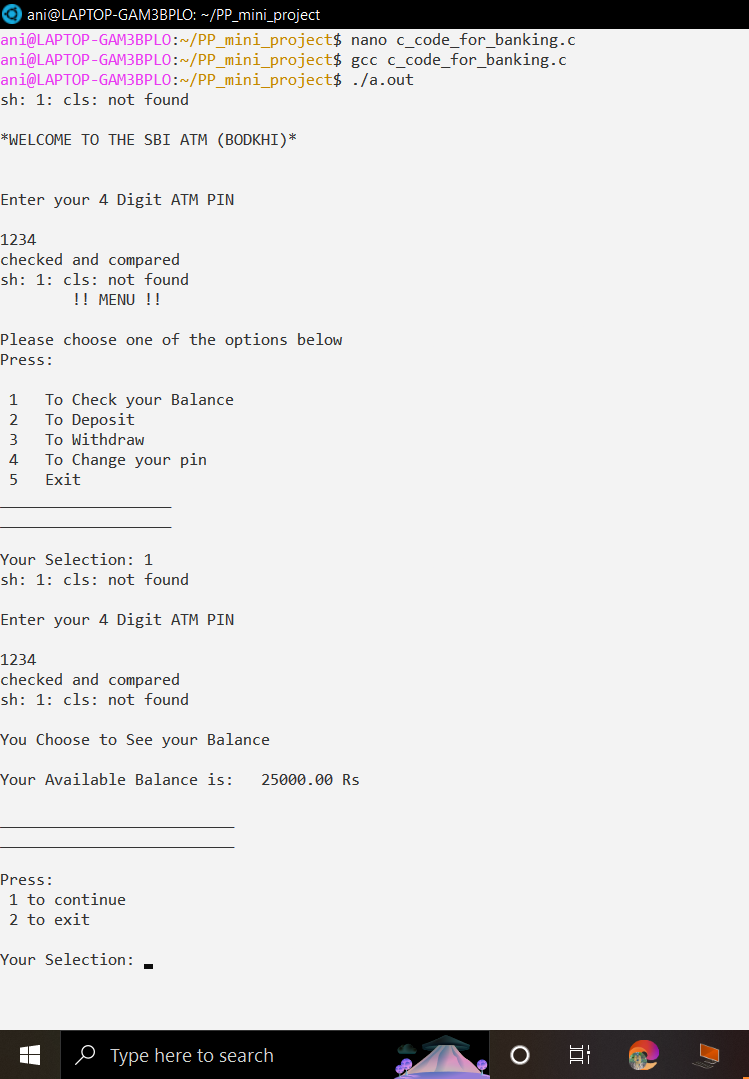
\includegraphics[scale=0.35]{output_c_1.png} \\ \\
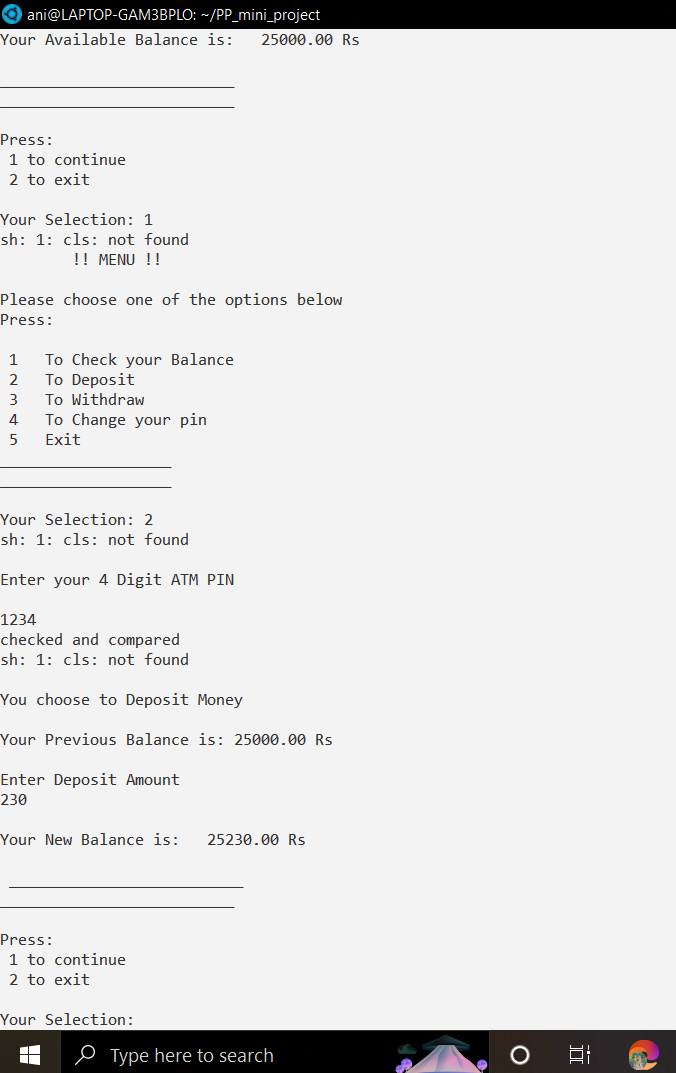
\includegraphics[scale=0.35]{output_c_2.png} \\

\section{Profiling}


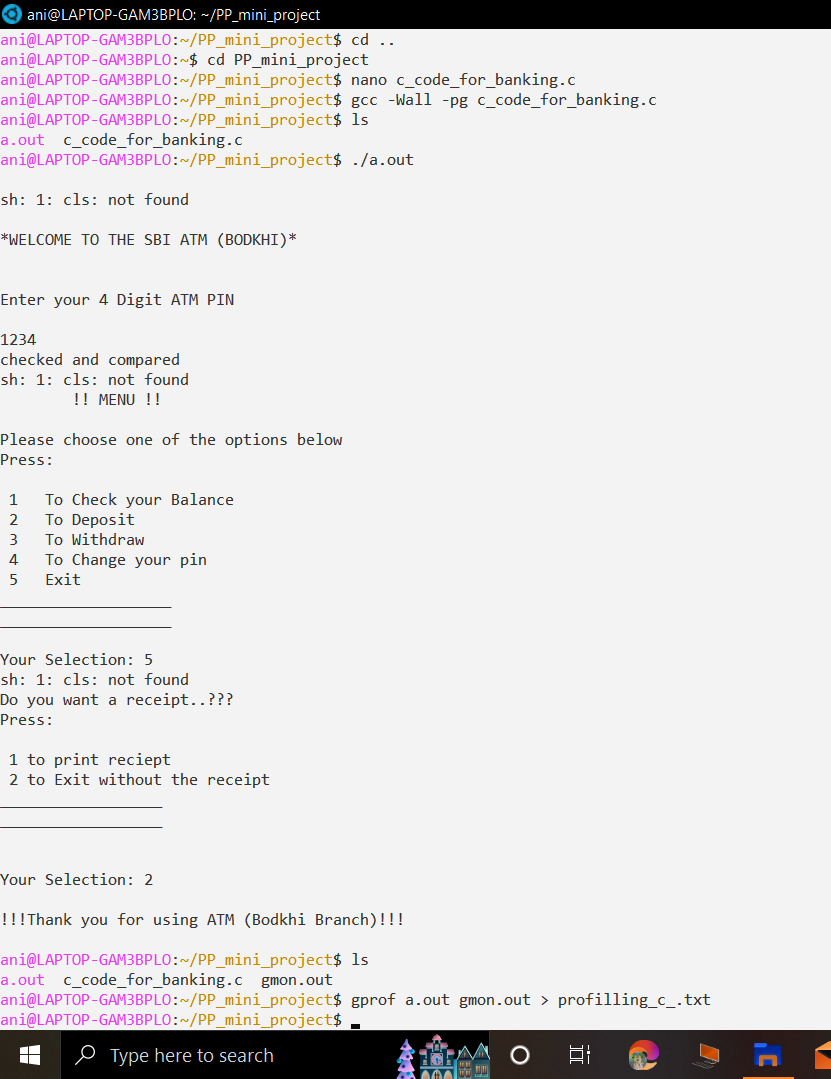
\includegraphics[scale=0.35]{profilling1.png} \\ \\
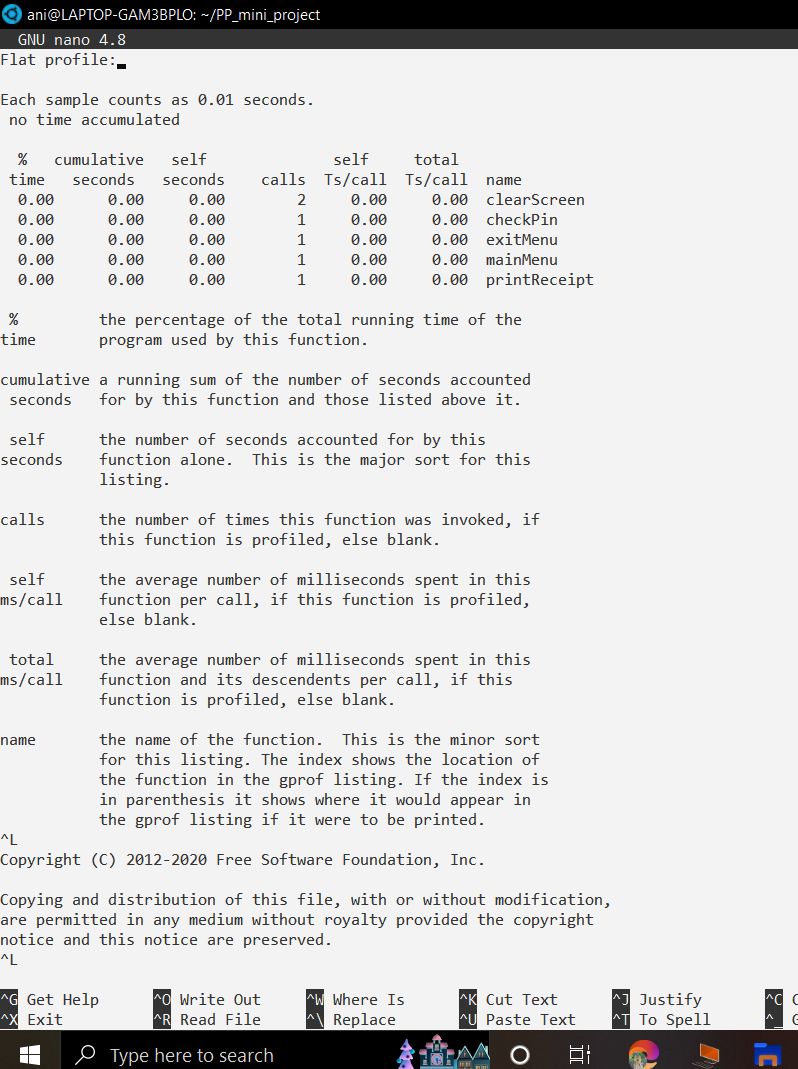
\includegraphics[scale=0.35]{profilling2.png} \\ \\
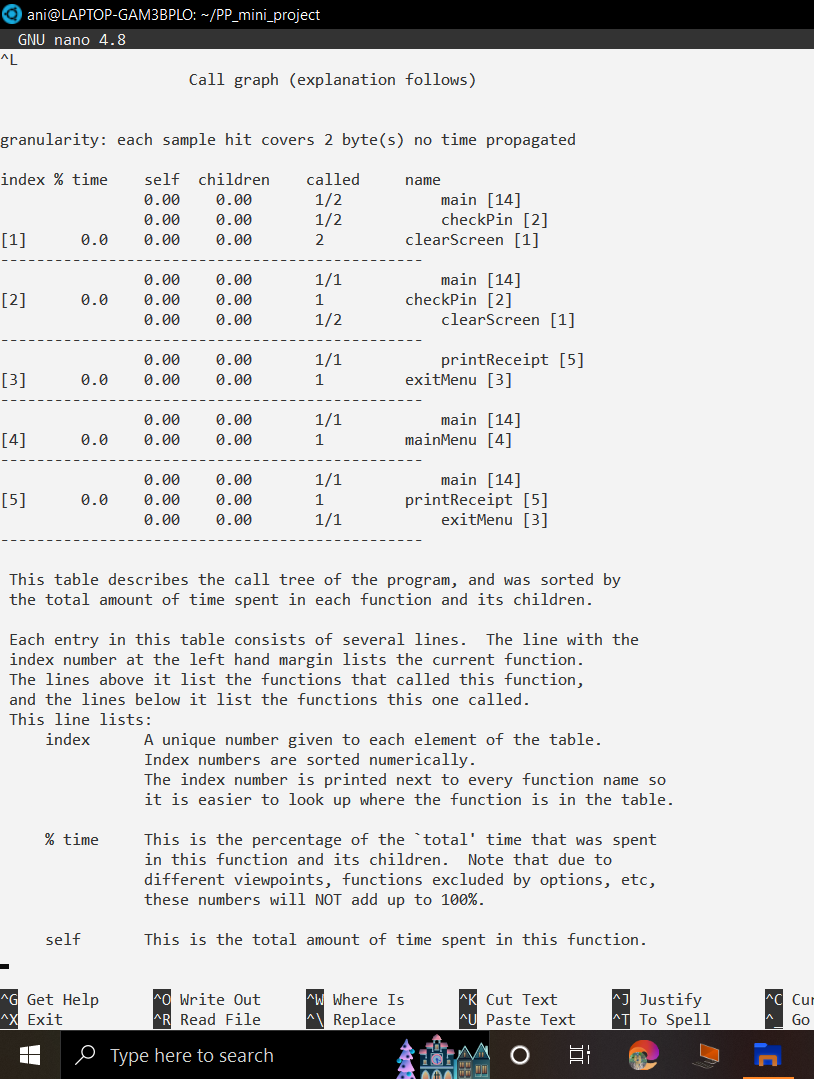
\includegraphics[scale=0.35]{profilling3.png} \\

\section{Debugging}


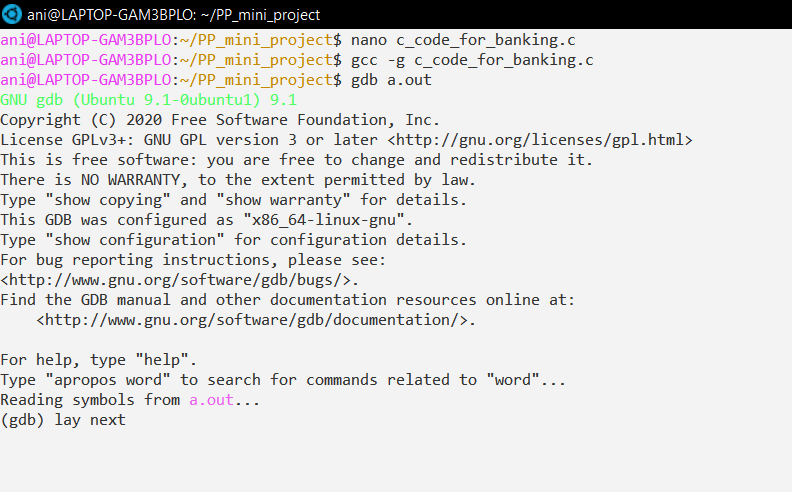
\includegraphics[scale=0.35]{debugging1.png}   \\ \\
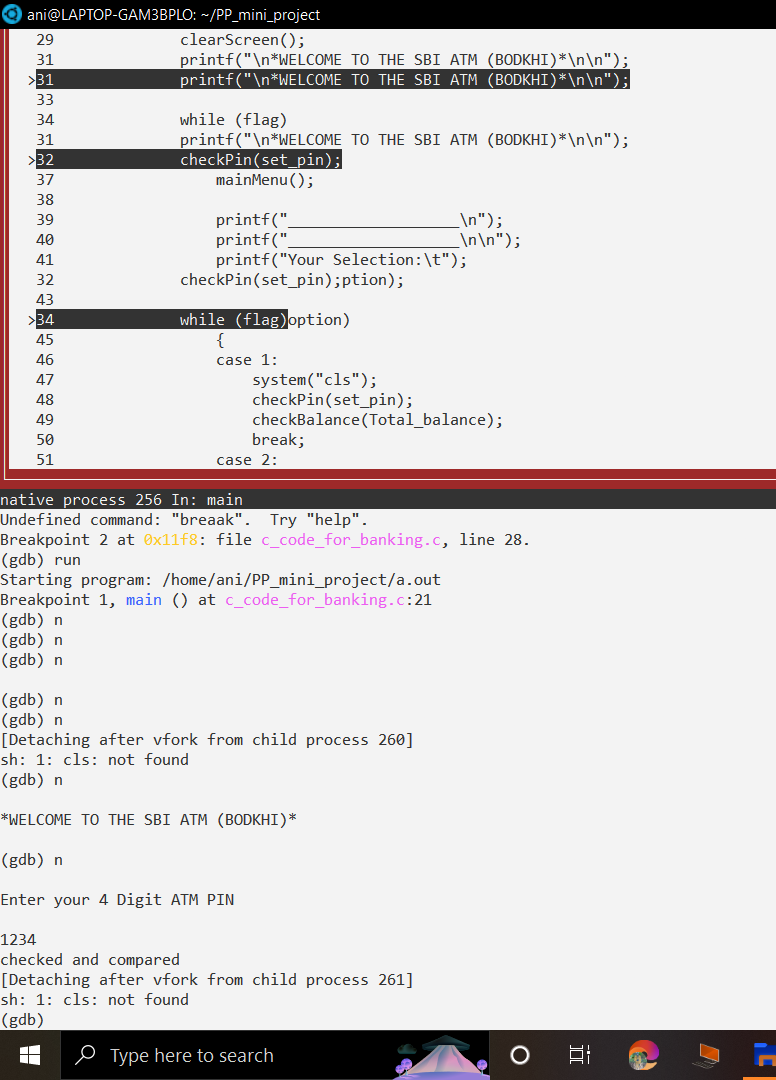
\includegraphics[scale=0.35]{debugging2.png}   \\ \\
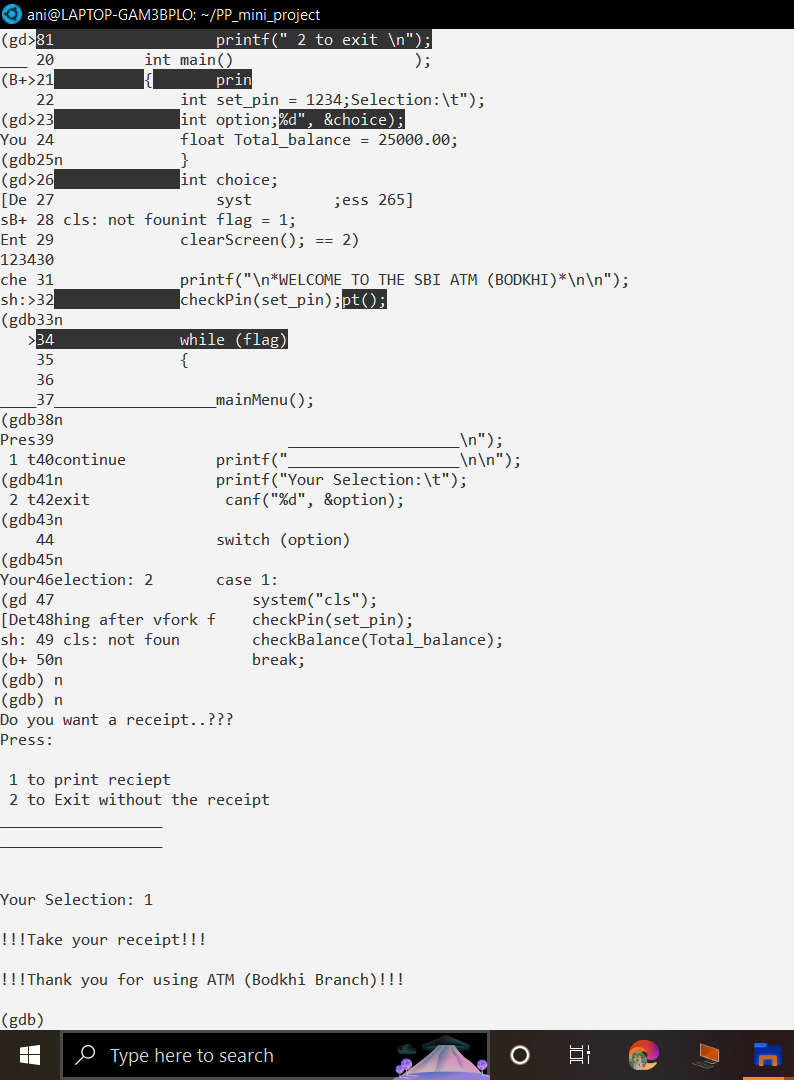
\includegraphics[scale=0.35]{debugging3.png}   \\ \\
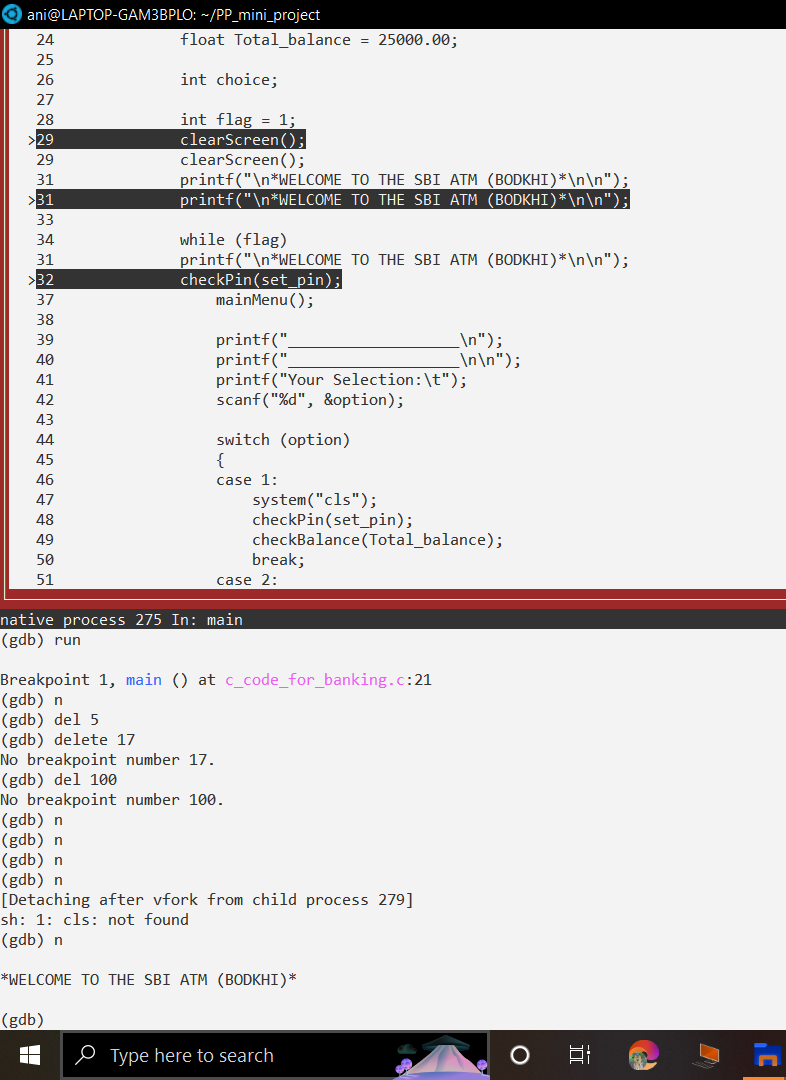
\includegraphics[scale=0.35]{debugging4.png}    \\ \\

\newpage

\section{Code In Python language:}

\begin{verbatim}[style=chstyle,language=Python]
import os

# Functions
# clearScreen()
# mainMenu()
# checkBalance(Total_balance)
# moneyDeposit(Total_balance)
# moneyWithdraw(Total_balance)
# printReceipt()
# exitMenu()
# errorMessage()
# checkPin()
# changePin()


# Main function !!!!

def main():

    Total_balance = 25000.00
    set_pin = 1234
    flag = True
    # clearScreen()
    print("\n***WELCOME TO THE SBI ATM (BODKHI)***\n")
    checkPin(set_pin)
    while (flag):

        mainMenu()

        print("____________________________")
        print("____________________________\n")
        print("Your Selection:\t", end="")

        option = int(input())

        # in place of switch cases in c code
        if option == 1:

            clearScreen()
            checkPin(set_pin)
            checkBalance(Total_balance)

        elif option == 2:

            clearScreen()
            checkPin(set_pin)
            Total_balance = moneyDeposit(Total_balance)

        elif option == 3:

            clearScreen()
            checkPin(set_pin)
            Total_balance = moneyWithdraw(Total_balance)

        elif option == 4:
            clearScreen()
            checkPin(set_pin)
            set_pin = changePin(set_pin)

        elif option == 5:

            clearScreen()
            printReceipt()
            return False

        else:
            errorMessage()

        print("_______________________________________")
        print("_______________________________________\n")

        print("Press:\n 1 to continue ")
        print(" 2 to exit \n")
        print("\nYour Selection:\t", end="")
        choice = int(input())
        os.system("cls")

        if (choice == 2):
            flag = False
            printReceipt()


# Defination of Functions

def mainMenu():
    print("\t!! MENU !!\n")
    print("Please choose one of the options below\nPress:\n")
    print(" 1   To Check your Balance")
    print(" 2   To Deposit")
    print(" 3   To Withdraw")
    print(" 4   To change your pin")
    print(" 5   Exit")


def clearScreen():
    os.system("cls")


def checkBalance(Total_balance):

    print("\nYou Choose to See your Balance\n")
    print(f"Your Available Balance is:  {Total_balance} Rs\n")


def moneyDeposit(Total_balance):

    print("\nYou choose to Deposit Money\n")
    print(f"Your Previous Balance is: {Total_balance} Rs\n")
    print("Enter Deposit Amount")
    deposit_amount = float(input())

    Total_balance += deposit_amount

    print(f"Your New Balance is:  {Total_balance} Rs\n ")
    return Total_balance


def moneyWithdraw(Total_balance):

    flag1 = True

    print("\nYou choose to Withdraw Money\n")
    print(f"Your Balance is: {Total_balance} Rs\n")

    while (flag1):

        print("Enter Withdraw Amount:\n")
        withdraw_amount = float(input())

        if (withdraw_amount <= Total_balance):

            flag1 = False
            Total_balance -= withdraw_amount
            print(f"\nYour withdrawing money is:  {withdraw_amount} Rs\n")
            print(f"Your New Balance is:  {Total_balance} Rs\n")

        else:
            clearScreen()
            print("!!INSUFFICIENT BALANCE!!\n")

            print(f"!!Your Account Balance is:  {Total_balance} Rs!!\n\n")

    return Total_balance


def printReceipt():

    print("Do you want a receipt..???\n")
    print("Press:\n\n 1 to print reciept\n 2 to Exit without the receipt \n")

    print("_____________________________________")
    print("_____________________________________\n")

    print("\nYour Selection:\t", end="")
    reciept = int(input())

    if (reciept == 1):

        print("\n!!!Take your receipt!!!\n")
        exitMenu()

    elif (reciept == 2):

        exitMenu()


def exitMenu():

    print("\n!!!Thank you for using ATM (Bodkhi Branch)!!!\n\n")


def errorMessage():

    print("!!!Invalid number!!!\n")


def checkPin(set_pin):

    print("\nEnter your 4 Digit ATM PIN\n")
    get_pin = int(input())
    if (set_pin == get_pin):

        print("checked and compared\n")
        clearScreen()

    else:

        print("\n!!!INCORRECT PIN!!!!\nTry AGAIN!!!!\n")
        checkPin(set_pin)


def changePin(set_pin):

    print("Enter new pin\n")
    new_pin = int(input())
    set_pin = new_pin
    print(f"Your new pin is : {set_pin}")

    return set_pin


main()

\end{verbatim}
\newpage
\section{Execution and Compilation}

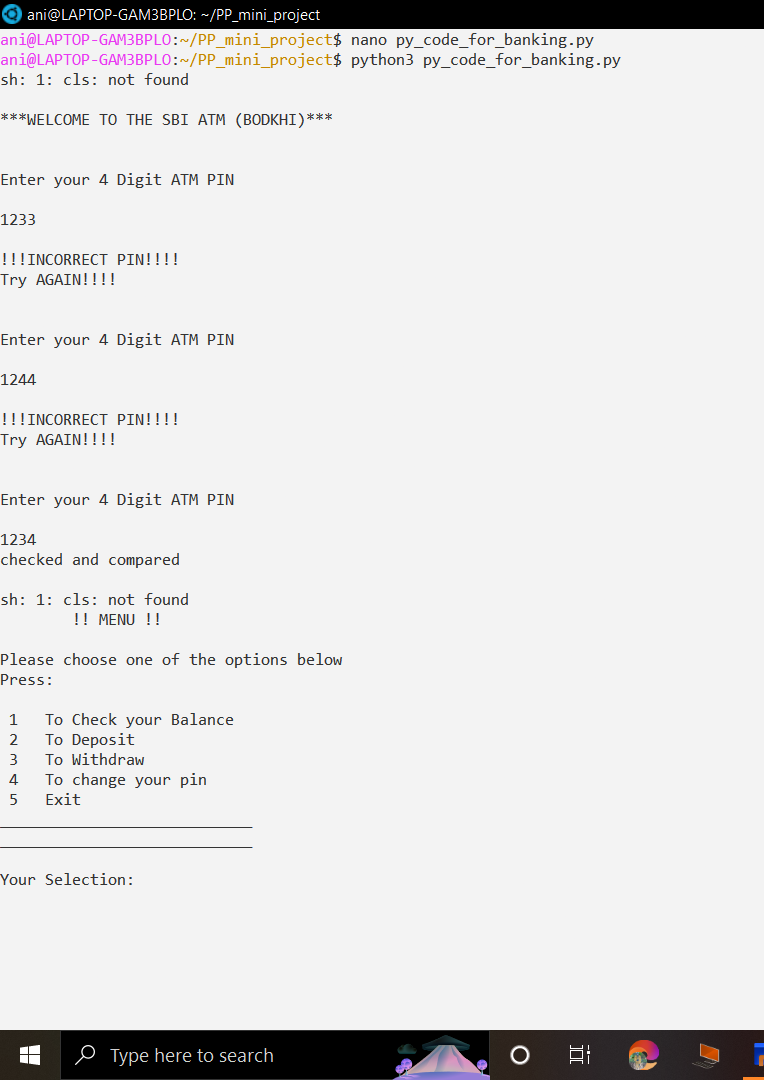
\includegraphics[scale=0.35]{output_py_1.png}  \\ \\
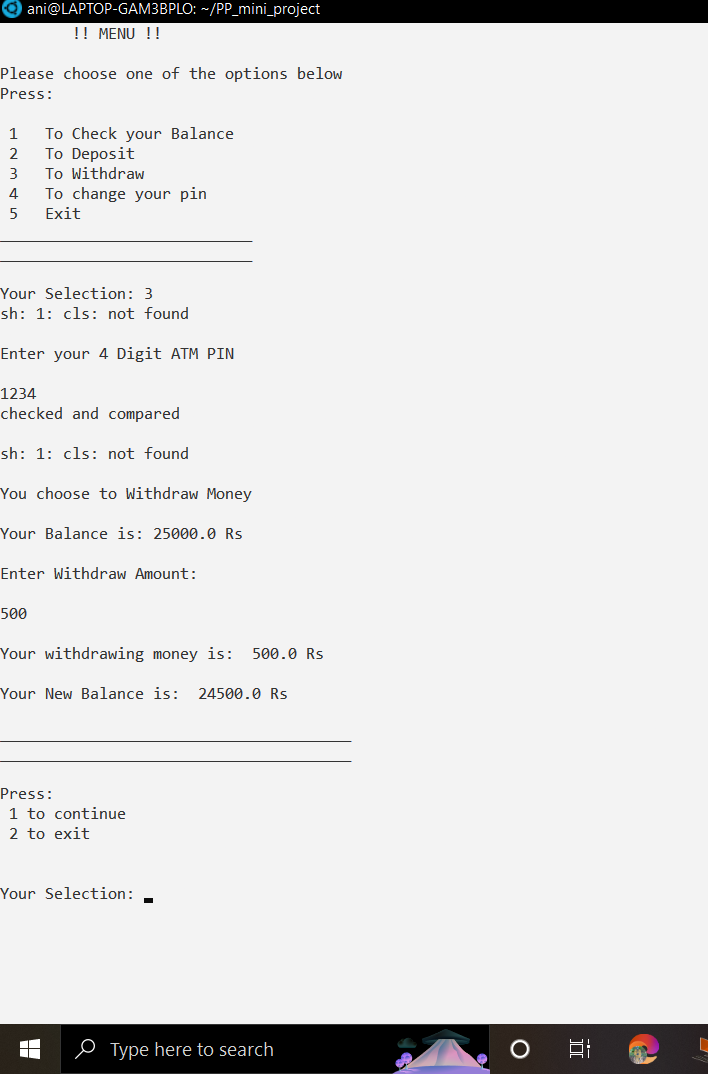
\includegraphics[scale=0.35]{output_py_2.png}  \\ \\
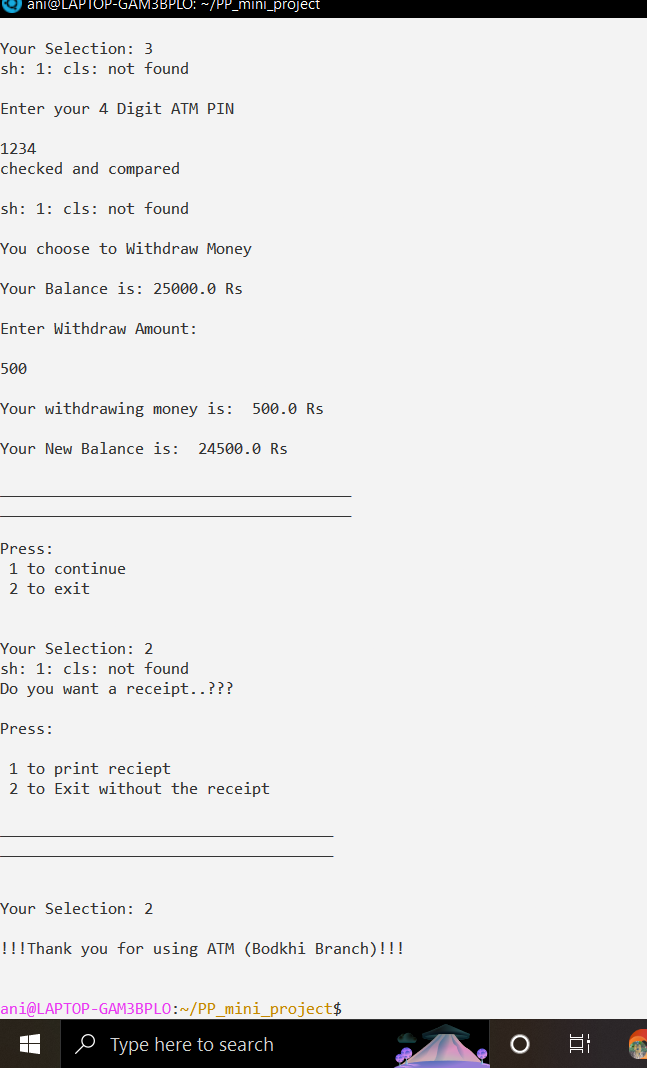
\includegraphics[scale=0.35]{output_py_3.png}  \\ \\

\section{Version Controlling}

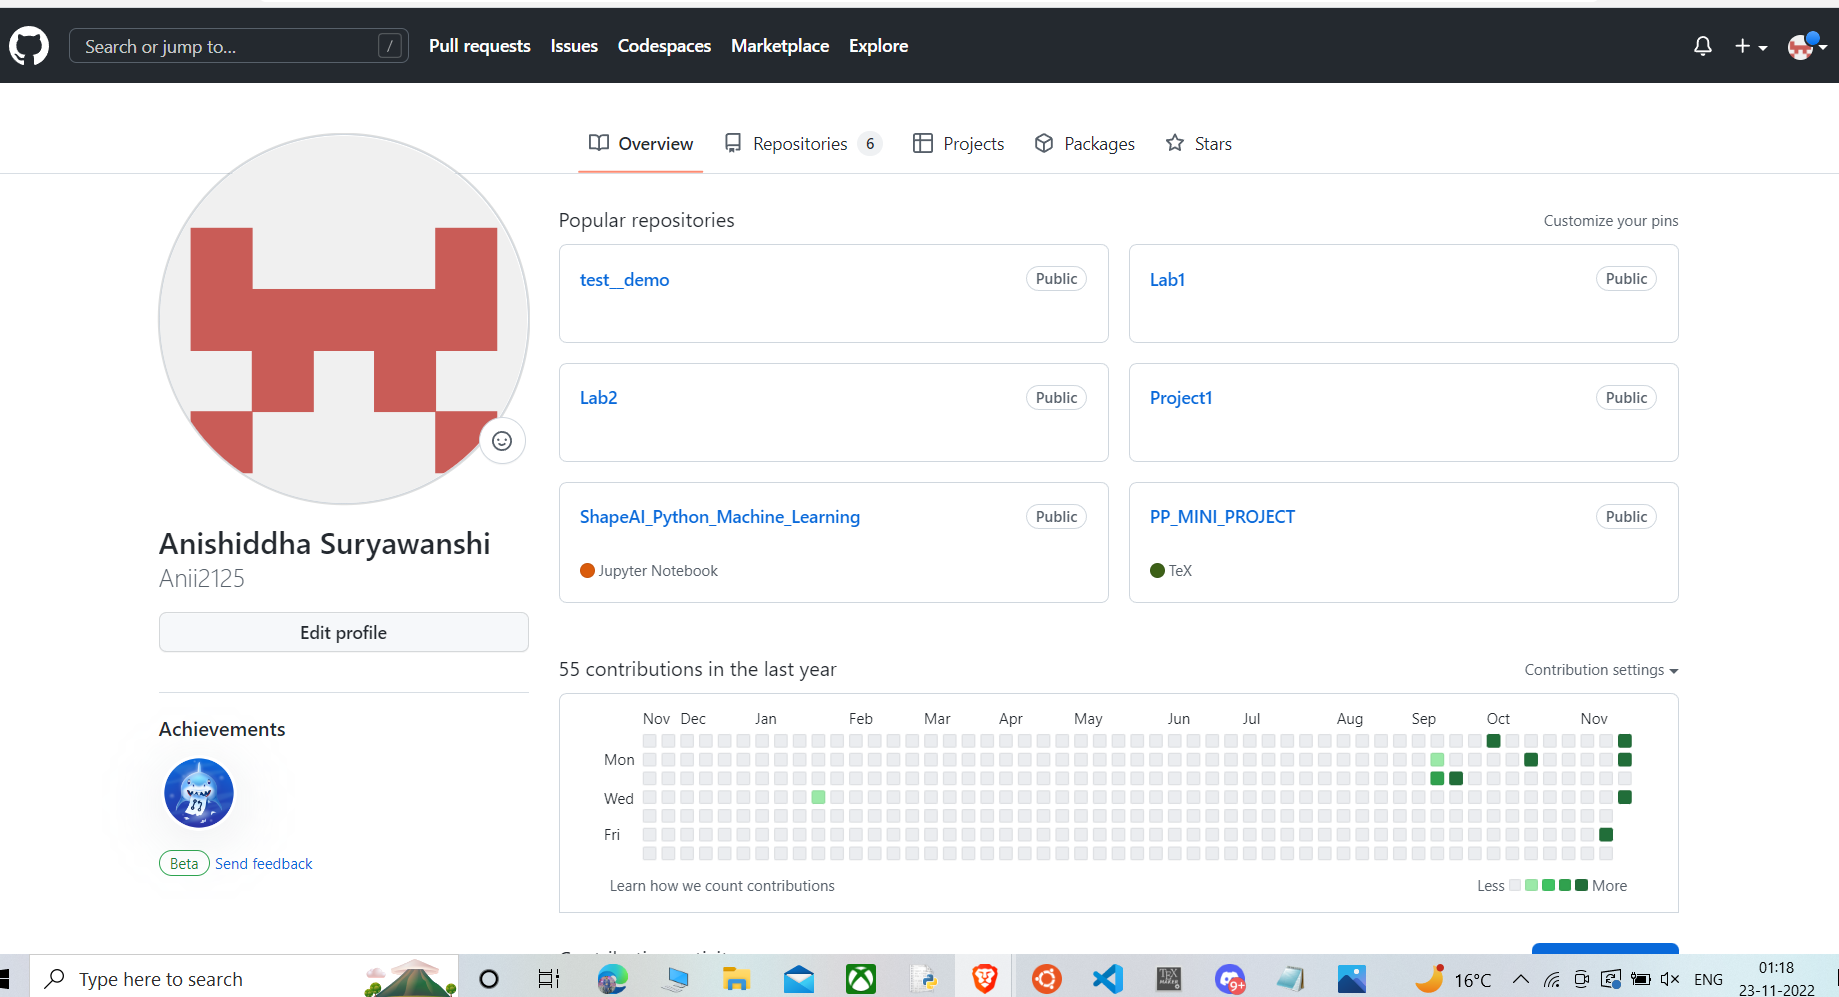
\includegraphics[scale=0.35]{github1.png}  \\ \\
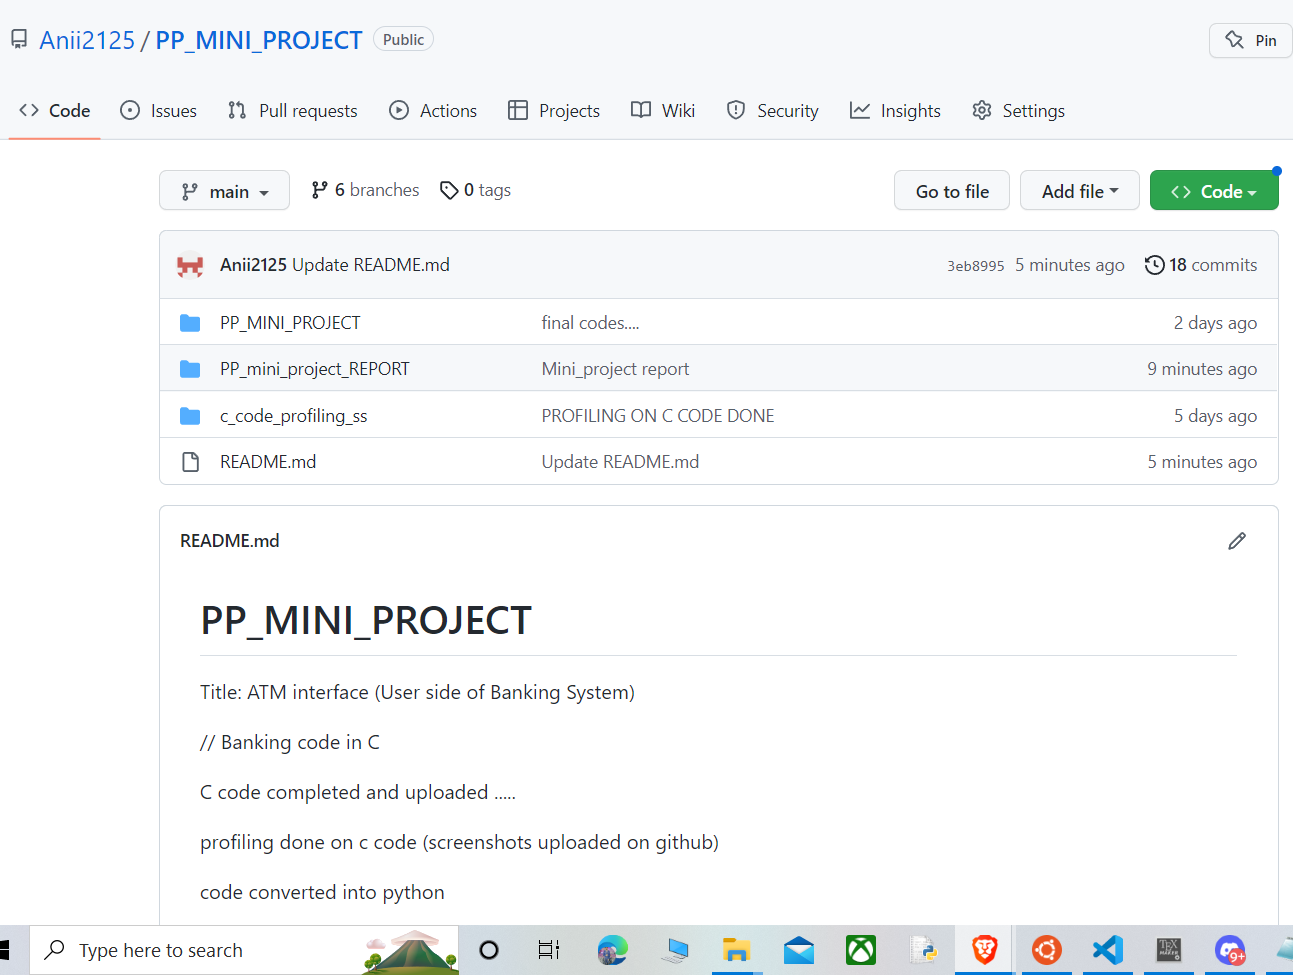
\includegraphics[scale=0.35]{github2.png}  \\ \\
    
 \end{document}